%for a more compact document, add the option openany to avoid
%starting all chapters on odd numbered pages
\documentclass[12pt]{cmuthesis}

% This is a template for a CMU thesis.  It is 18 pages without any content :-)
% The source for this is pulled from a variety of sources and people.
% Here's a partial list of people who may or may have not contributed:
%
%        bnoble   = Brian Noble
%        caruana  = Rich Caruana
%        colohan  = Chris Colohan
%        comar    = Cyrus Omar
%        jab      = Justin Boyan
%        josullvn = Joseph O'Sullivan
%        jrs      = Jonathan Shewchuk
%        kosak    = Corey Kosak
%        mjz      = Matt Zekauskas (mattz@cs)
%        pdinda   = Peter Dinda
%        pfr      = Patrick Riley
%        dkoes = David Koes (me)

% My main contribution is putting everything into a single class files and small
% template since I prefer this to some complicated sprawling directory tree with
% makefiles.

% some useful packages
\usepackage{times}
\usepackage{fullpage}
\usepackage{graphicx}
\usepackage{amsmath}
\usepackage[numbers,sort]{natbib}
\usepackage[backref,pageanchor=true,plainpages=false, pdfpagelabels, bookmarks,bookmarksnumbered,
%pdfborder=0 0 0,  %removes outlines around hyper links in online display
]{hyperref}
%\usepackage{subfigure}
\usepackage{caption}
\usepackage{subcaption}

\graphicspath{ {images/} }

% Approximately 1" margins, more space on binding side
%\usepackage[letterpaper,twoside,vscale=.8,hscale=.75,nomarginpar]{geometry}
%for general printing (not binding)
\usepackage[letterpaper,twoside,vscale=.8,hscale=.75,nomarginpar,hmarginratio=1:1]{geometry}

% Provides a draft mark at the top of the document. 
\draftstamp{\today}{DRAFT}

\begin {document} 
\frontmatter

%initialize page style, so contents come out right (see bot) -mjz
\pagestyle{empty}

\title{ %% {\it \huge Thesis Proposal}\\
{\bf Ground Up Design and Implementation of a Multi-modal Object Detection and Localization System}}
\author{Vasu Agrawal}
\date{\today}
\Year{2019}
\trnumber{still need to get TR number}

\committee{
Sebastian Scherer, Chair \\
Kris Kitani \\
Rogerio Bonatti
}

\support{}
\disclaimer{}

% copyright notice generated automatically from Year and author.
% permission added if \permission{} given.

\keywords{Stuff, More Stuff}

\maketitle

%\begin{dedication}
%For my dog
%\end{dedication}

\pagestyle{plain} % for toc, was empty

%% Obviously, it's probably a good idea to break the various sections of your thesis
%% into different files and input them into this file...

\begin{abstract}
\begin{enumerate}
	\item People (first responders and warfighters) need to gain rapid situational awareness about unknown subterranean environments.
	\item This is typically done by sending people in.
	\item These environments are very poor (rough terrain, terrible lighting, etc), making it difficult for standard robots / robot algorithms.
	\item This work presents the development of a multimodal object detection and localization system.
	\item Specifically, we cover the development of two iterations of a modular sensing platform, algorithms to detect and localize artifacts across multiple sensing modalities, and data transmission techniques to ensure timely updates for human operators.
	\item We show that the use of multiple sensors and sensing modalities is necessary and advantageous in detecting and localizing objects as a form of situational awareness in these difficult underground environments.
	\item Also, this localization system is aware of slam updates / key poses, and can maintain global consistency with the SLAM setup.
	\item Final evaluations are provided against the DARPA SubT challenge tunnel circuit environment ground truth.
\end{enumerate}
\end{abstract}

\begin{acknowledgments}
\begin{itemize}
	\item George
	\item Ratnesh
	\item thesis committee
	\item subt team / airlab
	\item kosbie / 112 squad
	\item roboclub people
	\item darpa subt challenge for paying for this?
	\item Justin also wanted to be acknowledged for putting up with me
\end{itemize}
\end{acknowledgments}

\tableofcontents
\listoffigures
\listoftables

\mainmatter

%% Double space document for easy review:
%\renewcommand{\baselinestretch}{1.66}\normalsize

% The other requirements Catherine has:
%
%  - avoid large margins.  She wants the thesis to use fewer pages, 
%    especially if it requires colour printing.
%
%  - The thesis should be formatted for double-sided printing.  This
%    means that all chapters, acknowledgements, table of contents, etc.
%    should start on odd numbered (right facing) pages.
%
%  - You need to use the department standard tech report title page.  I
%    have tried to ensure that the title page here conforms to this
%    standard.
%
%  - Use a nice serif font, such as Times Roman.  Sans serif looks bad.
%
% Other than that, just make it look good...

\chapter{Introduction}

Rapid situational awareness is crucial to enabling a successful response from first responders during an emergency. Incident command uses all information available to them to make decisions and coordinate the first responders. First responders are often sent into the incident scene to gather information, but the nature of emergencies makes this process dangerous and can risk additional lives \cite{whysubtmatters}. Subterranean environments pose a number of additional hazards and challenges, such as outdated maps, dangerous terrain, and low visibility, making them particularly difficult to send humans into safely. For example, emergency personnel cannot safely explore beyond fires in coal mines, and are thus unable to determine the number of people or quality of terrain that may be behind them \cite{mshapresentation}. Autonomous systems have the potential to significantly improve the quality and timeliness of the situational awareness gained in challenging subterranean environments, and by doing so can reduce risk to human lives.

\section{The DARPA Subterranean Challenge (SubT)}

The DARPA (Defense Advanced Research Projects Agency) Subterranean Challenge was issued to spur the development of new technologies for exploring complex underground environments. Teams are challenged to propose new and innovative solutions for the unique perception, mobility, communication, and autonomy problems present in these environments. Teams compete in a series of 3 separate circuit events, each in a different type of subterranean environment, listed in Figure \ref{darpa_environments}. The highest performing teams will be invited to a final event which incorporates elements of each type of environment. In each event, teams are tasked with deploying systems which rapidly provide situational awareness, in the form of map data and locations of predetermined objects placed by DARPA. Each object ("artifact") represents a particular class of objects which are likely to be found in subterranean environments, such as those shown in Figure \ref{tunnel artifacts}.

\begin{figure}	
	\centering
	\includegraphics[width=\textwidth]{darpa_environments.jpg}
	\caption[DARPA Subterranean Challenge environments]{The Tunnel Circuit focuses on human made tunnel systems. The Urban Circuit focuses on urban environments such as mass transit and municipal infrastructure. The Cave Circuit focuses on naturally occurring cave systems. Image from DARPA \cite{subtenvironments}.}
	\label{darpa_environments}
\end{figure}

During each circuit event, teams have 60 minutes to deploy their systems in the environment. The deployment may consist of as many robots as the teams desire, but must be operated by a single human supervisor at the team's base station. Not all areas of the environment will be traversable for all types of robots, so teams are encouraged to develop systems with a variety of mobility capabilities. Autonomous exploration capability is advised to reduce operator load and eliminate a need for constant connectivity. Communication with and coordination of each robot in the fleet is a challenge as no communication infrastructure is provided by DARPA.  The perception systems used to drive the autonomy should be able to handle a variety of challenging conditions, such as low visibility and variable lighting. This differs from typical perception benchmarks, such as ImageNet \cite{deng2009imagenet}, which ensure clean and high quality data. Teams may be permitted multiple runs per event.

Before a team's run, DARPA places a predetermined and disclosed number of artifacts in the environment. The locations of specific points on each of these artifacts, referenced to a DARPA-defined frame, are surveyed and treated as ground truth. The location of each artifact and number of each artifact type is unknown to teams. Scoring for each competition event is based entirely on the number of artifacts which are correctly reported to DARPA within the 60 minute period. Teams must report the artifact's category and must report coordinates which are within 5m Euclidean distance of the ground truth for an artifact report to be considered correct. Teams may submit twice the number of artifact reports as there are artifacts in the environment. Artifact reports may be generated in whichever manner a team deems appropriate, such as randomly, by the human supervisor, or fully autonomously by the deployed system. Ties between multiple teams are broken by a number of factors, including the times artifacts were submitted, and the furthest artifacts detected \cite{tunnel_rules}.

\section{Tunnel Circuit Specifics}

This work focuses specifically on artifact detection and localization in the context of the Tunnel Circuit. The Tunnel Circuit event took place between at the National Institute for Occupational Safety and Health Mining (NIOSH) site in Pittsburgh, PA, between August 15 and August 22 2019. DARPA divided the former coal mine into two separate courses, starting at the mine's two separate portals, Safety Research and Experimental. A map of the Safety Research course is shown in Figure \ref{tunnel_circuit_day_2}. Each team was allowed 2 runs in each course. The team's final score is a sum of the highest score from each course.

20 artifacts were deployed by DARPA in each course. The placement and distribution of artifacts varied between each course and each run, as indicated in Table \ref{final_scores}. Five specific categories of artifacts were used at the Tunnel Circuit. A single representative model of each artifact, shown in Figure \ref{tunnel artifacts}, was used. Specific model numbers for each representative object were distributed to teams in advance of the competition \cite{tunnel_artifacts}.

\subsubsection{Backpack}

The backpack artifact represents a typical adult-sized bag for carrying items. The backpack may be found on the ground, on a wall, or resting on a work surface, such as a table. The backpack contains a sandbag to help keep it in place during the competition. The front backpack is facing outward or upward depending on the initial placement.

\subsubsection{Cell Phone}

The cell phone artifact represents a radio used for communication, as well as other typical handheld devices. The cell phone is playing an unspecified full-screen video. Audio is playing from the phone at maximum volume. A 2.4 GHz access point is created by each cell artifact with an SSID of the form "PhoneArtifact\#\#", where "\#\#" is a unique two digit number. The cell phone's Bluetooth radio is on and discoverable.

\subsubsection{Drill}

The drill artifact represents a typical handheld tool. The drill has a Philips head driver in its chuck. The artifact may be found on the ground or on work tables. The orientation of the drill is not specified. The drill is not powered during scored runs.

\subsubsection{Fire Extinguisher}

The fire extinguisher artifact represents a typical common handheld fire extinguisher. This artifact also represents areas where other emergency equipment may be located. The fire extinguisher has its hose in the stored configuration. It may be found on the ground, on a work surface, or hanging from a wall. It will not be used during the scored runs.

\subsubsection{Survivor ("Randy")}

The survivor artifact represents a human survivor, such as a trapped worker. A thermal manikin is used, and is wearing a high visibility jacket, work pants, and standard steel toed work boots. The manikin has heating elements in its hands and head to partially emulate a human's thermal signature. The manikin is not actuated and does not play auditory clues. The manikin is placed in a static sitting position against walls.

\begin{figure}
	\centering
	\begin{subfigure}{0.32\textwidth}
		\includegraphics[width=\textwidth,height=5.5cm,keepaspectratio]{backpack_artifact.png}
		\caption{Backpack}
		\label{backpack}		
	\end{subfigure}
	\hfill
	\begin{subfigure}{0.32\textwidth}
		\includegraphics[width=\textwidth,height=5.5cm,keepaspectratio]{cell_phone_artifact.png}
		\caption{Cell Phone}
		\label{cell phone}
	\end{subfigure}	
	\hfill
	\begin{subfigure}{0.32\textwidth}
		\includegraphics[width=\textwidth,height=5.5cm,keepaspectratio]{drill_artifact.png}
		\caption{Drill}
		\label{drill}
	\end{subfigure}
	\\
	\begin{subfigure}{0.32\textwidth}
		\includegraphics[width=\textwidth,height=5.5cm,keepaspectratio]{fire_extinguisher_artifact.png}
		\caption{Fire Extinguisher}
		\label{fire extinguisher}
	\end{subfigure}
	\begin{subfigure}{0.32\textwidth}
		\includegraphics[width=\textwidth,height=5.5cm,keepaspectratio]{randy_artifact.png}
		\caption{Survivor ("Randy")}
		\label{randy}
	\end{subfigure}	
	\caption[Tunnel Circuit artifacts]{The Figure depicts the 5 Tunnel Circuit artifacts. The survivor, cell phone, and backpack artifacts are common to all 3 circuit events. Each circuit consists of an additional 2 circuit-specific artifacts, which were the fire extinguisher and drill for the Tunnel Circuit. All 9 artifacts will be used during the final event. The localization point in the images is the specific point surveyed by DARPA against which error will be measured. Images from DARPA \cite{tunnel_artifacts}.}
	\label{tunnel artifacts}
\end{figure}

\section{Our Approach}

Our team's overall concept of operations is one of modular autonomy. We aim to develop a set of hardware and software components that can be rapidly reconfigured and adapted to support the needs of any particular environment. Individual modules can be upgraded or replaced as necessary. For mobility, modules such as removable battery packs, wheel assemblies, and drive electronics are used. These mechanical modules combined to form 3 robots during the Tunnel Circuit -- R1, a fixed body ground robot, R2, a ground robot with a center pivot body, and D1, a hexcopter. For communication, custom nodes are developed, multiples of which can be stored on modular node dropper assemblies. R1 and R2 each carried a node dropper during the Tunnel Circuit. For perception, this approach means the development of various sensing payloads with integrated software and computation that can be transferred between robots. These sensing payloads run modular state estimation and artifact detection and localization software which can adapt to the capabilities of each system. R1, R2, and D1 each had separate sensing payloads -- Mk. 0, Mk. 1, and Drone payload, respectively.

Within each sensing payload, we use a multimodal suite of sensors for artifact detection. Though a single sensor or category of sensors, such as RGB cameras, may be able to detect multiple types of artifacts, it is unlikely to be able to perform well in all conditions. Alternatively, individual sensors may be particularly well suited to detect a specific artifact easily, but may not detect others at all. For example, the survivor and cell phone artifacts emit a thermal signature that may be able to be detected in a thermal camera, leading to the localization of these artifacts even in cases of little to no light. A WiFi radio may be used to detect and localize which is beyond line of sight, but is incapable of detecting any other categories of artifacts. Using a multimodal suite of sensors with intelligent fusion allows us to exploit the strengths of each individual sensor and create a more accurate and robust overall system.

The human supervisor is also considered a module in our system. Though each robot in the system is capable of autonomous operation, the human supervisor is able to combine course and map information reported from multiple robots and direct the exploration patterns of the fleet. Each robot also returns artifact information to the base station, which the human supervisor aggregates and verifies. Artifacts reports which have been approved by the human supervisor are sent to DARPA at the human supervisor's discretion, and are modified and resubmitted as more information becomes available if necessary. An overview of our approach is shown in Figure \ref{approach}.

\begin{figure}	
	\centering
	\includegraphics[width=\textwidth]{approach.png}
	\caption[Our approach]{Multiple robots explore the mine and deploy communication nodes as they go along. They report artifacts they detect to the human supervisor over the deployed network. The human supervisor verifies the artifacts and sends verified ones to DARPA. DARPA scores the artifacts and returns score updates. The human supervisor uses score updates, as well as other map information received from the robots, to guide autonomous exploration with waypoints.}
	\label{approach}
\end{figure}

\section{Related Work}

This work draws inspiration from and extends upon two areas of work -- subterranean mobile robots and multimodal object detection. The early 2000s saw the development of a number of robots intended for use in subterranean environments, such as CMU's Groundhog \cite{ferguson2004autonomous} and CSIRO's Numbat \cite{ralston1998numbat}. These robots were built to specifically address mobility and perception challenges presented by underground mines. They demonstrated considerable mobility in a variety of field experiments, but were limited in their autonomous capabilities by the available compute and sensing technologies \cite{morris2006recent}. Recent advancements in these areas have led to impressive state of the art results in a variety of areas of robot perception, as demonstrated in various tasks on datasets such as ImageNet \cite{deng2009imagenet}, COCO \cite{lin2014microsoft}, and KITTI \cite{Geiger2013IJRR}. Of particular relevance is multimodal object detection, which has seen recent interest due to the necessity for accurate perception by self driving cars in all conditions \cite{feng2019deep}.

\subsection{Subterranean Mobile Robots}

Early subterranean mobile robots like Groundhog were limited in the rapid situational awareness they could provide a basestation operator. Groundhog carried two scanning lasers for mapping and navigation, along with a gyroscope, encoders, and tilt sensors for odometry. 2D maps were generated on board and continually optimized to ensure global consistency, but were not reported to the base station due to a lack of communication infrastructure. The maps could be queried from recorded data after Groundhog returned. Though the fidelity of the maps was high enough to be useful for situational awareness, the high latency of the information could be costly in a disaster response scenario. Even after a base station operator downloaded the maps from the robot, searching the point clouds for specific objects would be a time consuming and inaccurate process done manually.

Other subterranean robots attempted to solve the communication problem with a tether. This enabled robots, such as the MSHA (Mine Safety and Health Administration) Andros V-2, to report video feeds to the base station in real time. The remote camera acted as a source of more rapid situational awareness than the point clouds from Groundhog, and provided data in a format more easily understandable by humans. However, tethers proved to be unreliable, being prone to tangling and breakage \cite{murphy2009mobile}, and thus unsuitable for disaster response scenarios which require robust solutions. Utilizing such a video streaming system for situational awareness may also prove difficult to scale to multiple robots as human operators would be required to split attention between multiple video feeds and thus potentially miss important moments.

Our work addresses many of the limitations of early systems for providing situational awareness. Each deployed robot in our system autonomously identifies important objects and sends it to the base station over a wireless link. Providing artifacts for situational awareness ensures that the human supervisor receives only high utility information, and reduces the difficulty of operating multiple robots covering a large environment at once. The small size of each artifact also enables transmission over a wireless link even when only low bitrates are available, ensuring real time updates.

\subsection{Multimodal Object Detection}

Multimodal object detection is an important problem for robots as it has the potential to enable more robust perception than any single sensor could. This is especially true for self driving cars, where human lives are at risk. The current best known methods for 2D and 3D object detection, as measured on the KITTI dataset, use deep learning to fuse LIDAR and RGB camera data. \cite{qi2018frustum} performs 2D object detection in RGB images and then projects and refines detections into 3D using LIDAR information. \cite{liang2019multi} instead jointly extracts features from LIDAR and RGB camera data and performs ROI feature fusion.

Unfortunately, these deep fusion methods rely on the availability of large, well labeled datasets to develop high accuracy, and require powerful GPUs to run in real time. Our approach differs by instead using deep learning techniques only to extract 2D bounding boxes from images, which can be done with relatively little training data, and fusing detections with other sensors using classical techniques. Our method for fusing detections from multiple sensing modalities requires only coordinates for each artifact. This allows for the use of additional detection techniques, such as cell phone trilateration \cite{iglesias2012indoor} and sound source localization \cite{grondin2019lightweight}. Work which directly fuses audio and signal strength data in a deep network with LIDAR and RGB data was not found in the literature.
\chapter{Hardware Development}

One of the cornerstones of our team's Concept of Operations for the SubT Challenge was modular autonomy. That is, we wanted to develop a series of modules which could be composed and rapidly reconfigured to suit the task at hand. The use of individual modules would also allow for components to be replaced or upgraded as necessary. For example, each of our ground robots had 4 drive modules, each consisting of a wheel, motor, gearbox, and a separate electronics module. The drive modules could be replaced or upgraded as necessary, such as in the case of a gearbox failing or the selection of different desired torque profiles. Similarly, we wanted to develop modular sensing and compute payloads which could be transferred across different robots, including in between ground and aerial robots, and which would be capable of performing all of the robot's high level autonomy functions.

Early indication that our approach should be feasible came as the result of using a prototype state estimation payload ("Blue Payload") similar to the Kaarta Traak \cite{kaarta_traak}. The payload was relatively small, self-contained, and could be easily transferred between robots (see Figure \ref{blue payload robots}). We simply had to mount the payload to the robot, apply power, and connect to the robot's internal network, and all of the payload's autonomy functions would be enabled. Overall, we found the Blue Payload quite simple to integrate, and wanted our future payloads to be similar in this regard. Inspired by the Blue Payload, and keeping the SubT Challenge requirements and timeline in mind, we came up with a list of some design goals and desired capabilities for our first payload ("Mk 0"), sorted by priority:

\begin{description}
	\item[Self-contained] All of the sensing and computation for the high level autonomy features should happen inside the payload itself. Ideally, the payload would only be supplied power and a network connection, just like the Blue Payload, and would output autonomy goals (such as waypoints) and information (such as robot state, maps, and artifact locations) to be relayed to the human supervisor at the base station.
	\item[Rapid Development] From the beginning of the competition (September 2018) to the first qualification deadline (December 2018), we had a little under 3 months to develop our first payload. This meant that, wherever possible, we should prefer designs that relied on existing expertise, such as the use of familiar components and sensors, and preferring in-house manufacturing capabilities with short lead times.
	\item[Environmentally Robust] We expected the field environments for the SubT competition to be somewhat hostile to the sensors. Specifically, we were told that "dust, fog, mist, water, and smoke are within scope" \cite{tunnel_rules}, and we wanted our payload to be reasonably protected against these elements, within reason. Additionally, the payload needed to be robust to the mechanical loading it would be subject to as a result of the rough terrain.
	\item[Weight Sensitivity] Similar to the Blue Payload, we wanted our new payload to be light enough to be carried by one of our aerial robots (as in Figure \ref{d1 blue payload}), or a smaller ground robot (as in Figure \ref{joeybot blue payload}) in addition to larger robots (as in Figure \ref{r1 blue payload}).
	\item[Low Cost] While there aren't specific restrictions on the maximum cost of our robot, DARPA was interested in identifying cost effective solutions for the SubT Challenge. Minimizing cost is also useful as a design goal as we intended to build multiple copies of the payload for our various robots, as well as to have spares.
\end{description}

\begin{figure}
	\centering
	\begin{subfigure}{0.3\textwidth}
		\includegraphics[width=\textwidth]{blue_payload_joeybot.png}
		\caption{Joeybot with Blue Payload}
		\label{joeybot blue payload}
	\end{subfigure}		
	\hfill
	\begin{subfigure}{0.3\textwidth}
		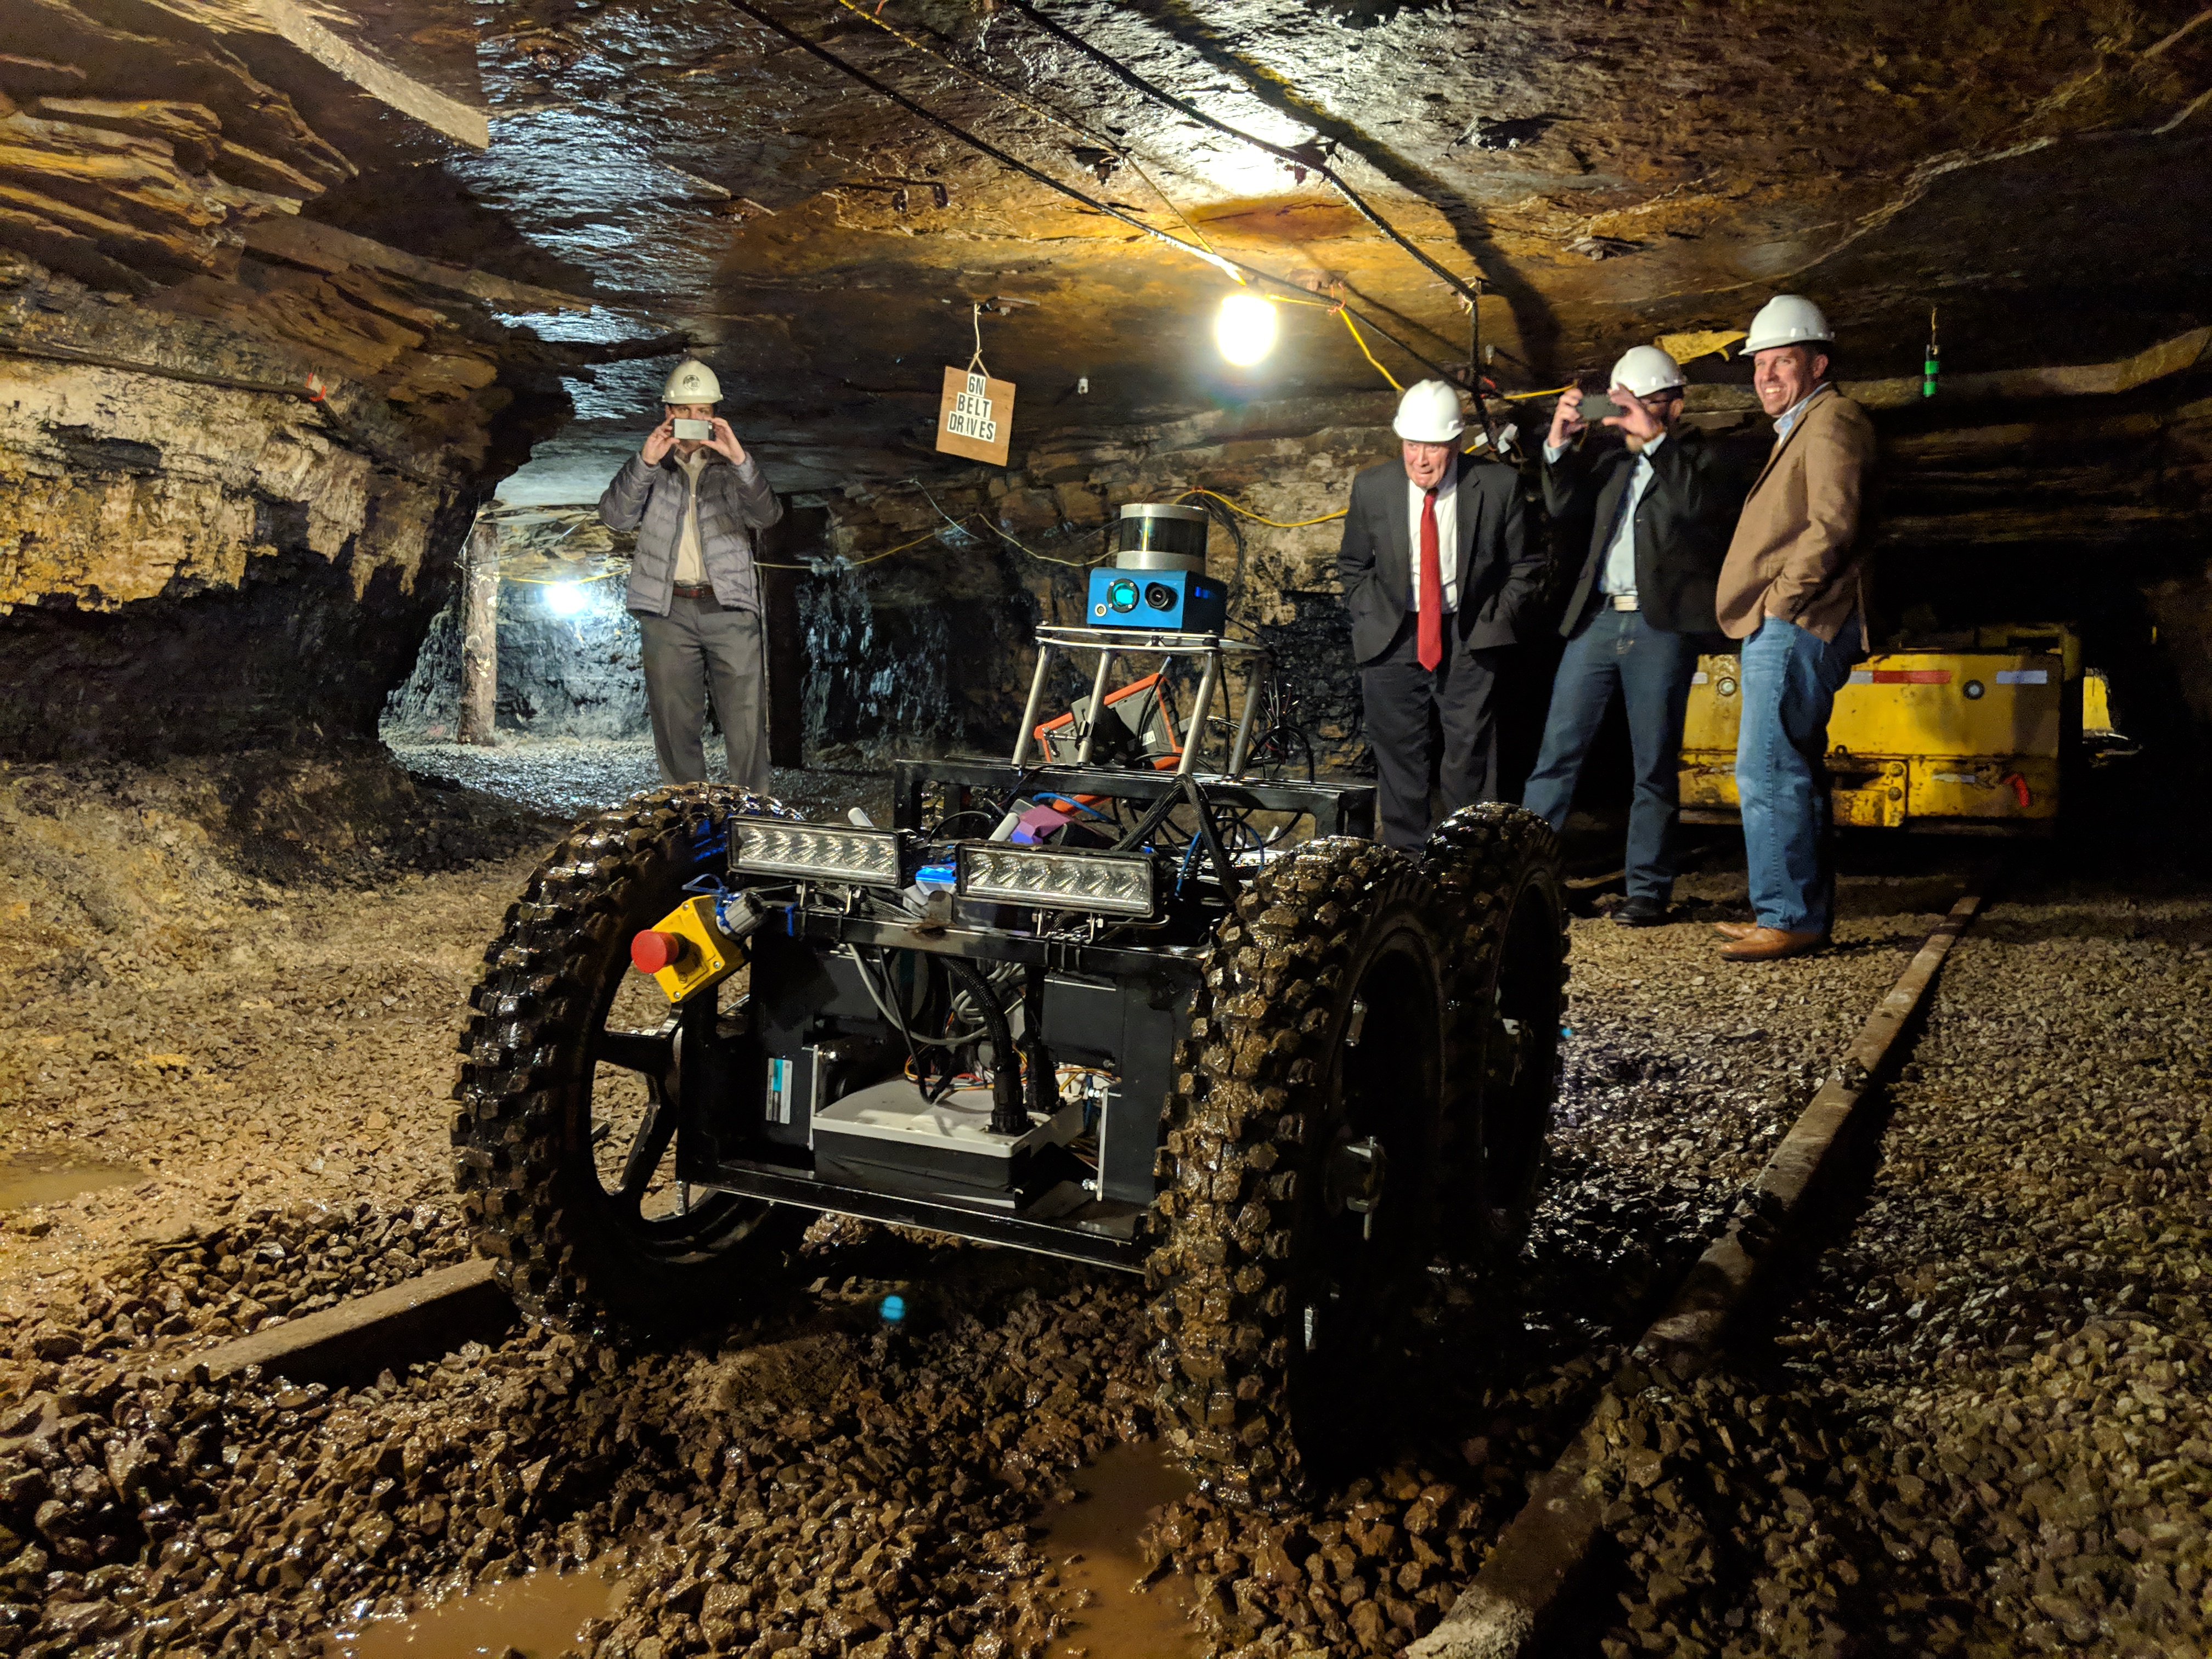
\includegraphics[width=\textwidth]{r1_with_blue_payload.jpg}
		\caption{R1 with Blue Payload}
		\label{r1 blue payload}		
	\end{subfigure}
	\hfill
	\begin{subfigure}{0.3\textwidth}
		\includegraphics[width=\textwidth]{drone_with_blue_payload.png}
		\caption{D1 with Blue Payload}
		\label{d1 blue payload}
	\end{subfigure}	
	\caption{Robots with initial modular payload ("Blue Payload")}
	\label{blue payload robots}
\end{figure}

\section{Mk. 0 Component Selection}

\subsection{Computers}

In order to select the computer(s) to be used inside Mk. 0, it was important for us to figure out the tasks that the payload would need to perform. While we wouldn't be able to know exactly how many resources each of the tasks would consume, prior experience could help us determine some rough approximations. The main tasks for the payload would be the following:

\begin{enumerate}
	\item State estimation
	\item Path planning and navigation
	\item Object detection and localization
\end{enumerate}

For state estimation, we knew that we would be using LOAM \cite{zhang2014loam}, which was written by Ji Zhang (one of our team members), and is the current state of the art for SLAM. We knew that LOAM ran well on the Blue Payload, which uses an Intel NUC with an Intel Core i7 processor internally. The path planning and navigation stack was being actively developed and ran on the second computer on Joeybot (see Figure \ref{joeybot blue payload}), which was a mid-range industrial-grade PC from Logic Supply. Though the Logic Supply computer was also using an Intel Core i7 processor, the processor itself was underclocked to reduce heat output. Profiling indicated that it should be possible to run the path planning and navigation stack on the NUC being used to run LOAM, especially given the underclocked processor in the Logic Supply computer. This factor, along with various team members' familiarity with the NUC family of products, marked the Intel NUC as a strong contender for use in our payload. Specifically, we considered the NUC8i7BEB, which the best (with regards to CPU) available NUC board at the time.

Working under the assumption that we'd use an Intel NUC inside the payload, the question of running the object detection and localization stack still remained. While it wasn't yet clear what our object detection strategy would be, the use of convolutional neural networks in advancing the state of the art for object detection suggested that they would be a component of our approach. To efficiently run convolutional neural networks, a few hardware platforms were considered. We attempted to find a platform which we thought could run multiple neural networks in parallel, at relatively high frequencies (10+ Hz). We considered the following options:

\begin{enumerate}
	\item Intel Movidius Neural Compute Stick
	\item NUC8i7BEB integrated GPU (Intel Iris Plus Graphics 655)
	\item Nvidia Jetson TX2
	\item Nvidia Jetson AGX Xavier
\end{enumerate}

Of the available options, the Nvidia Jetson AGX Xavier ("Xavier") offered the highest inference performance due to its many CUDA cores, as well as its specialized Tensor Cores and Deep Learning Accelerators. Combined, the Xavier was capable of performing more than an order of magnitude more FLOPS than the other platforms. As we were unsure of the exact requirements of our object detection system at the time, we chose to overprovision, and thus the available FLOPS became the deciding factor. The Xavier emerged as the clear winner for our GPU selection inside the Mk. 0 payload. At this stage, it was also decided to commit to using the NUC8i7BEB inside Mk. 0. In an attempt to simplify the system, we briefly considered attempting to run the entire autonomy stack on a single Xavier, rather than split between a NUC and an Xavier. However, we felt that the slower ARM cores on the Xavier would not be able to handle the combined autonomy stack, and thus decided to continue using both computers inside the Mk. 0 payload. The NUC would handle the state estimation and path planning and navigation tasks while all object detection and localization tasks would run on the Xavier.

After the completion of the Mk. 0 payload, we performed some experiments to see if our earlier hypothesis about the Xavier being unable to handle the entire autonomy stack was correct. Profiling of the NUC revealed that LOAM was one of the heaviest processes, consuming nearly 100\% of a single core in some circumstances, and smaller portions of other cores. Thus, we decided to attempt to run LOAM on the Xavier first. For our benchmarking, we set up an Xavier Developer Kit in MAX-N mode after having disabled the frequency governors with the provided jetson\_clocks.sh script. This mode enables all of the processors in the Xavier, and pins them at their highest frequency. We attempted to run LOAM on pre-recorded data in a few different configurations, varying a parameter to adjust downsampling of the input point clouds to reduce the scan alignment cost. Figure \ref{loam_xavier} shows a visualization of the results.

\begin{figure}
	\centering
	\begin{subfigure}{0.3\textwidth}
		\includegraphics[width=\textwidth]{tour_ed_mine_1-00.png}
		\caption{100\% Point Cloud Scaling}
		\label{loam_xavier_100}
	\end{subfigure}		
	\hfill
	\begin{subfigure}{0.3\textwidth}
		\includegraphics[width=\textwidth]{tour_ed_mine_1-00_1-25s.png}
		\caption{75\% Point Cloud Scaling}
		\label{loam_xavier_75}		
	\end{subfigure}
	\hfill
	\begin{subfigure}{0.3\textwidth}
		\includegraphics[width=\textwidth]{tour_ed_mine_1-00_1-50s.png}
		\caption{50\% Point Cloud Scaling}
		\label{loam_xavier_50}
	\end{subfigure}	
	\caption[Visualization of LOAM running on an Xavier]{Visualization of LOAM running on an Xavier with different downsampling parameters, using pre-recorded data collected at the Tour-Ed Mine in Tarentum, PA.}
	\label{loam_xavier}
\end{figure}

In Figure \ref{loam_xavier_100}, the same configuration as the NUC on Mk. 0 was used. Severe misalignment is visible - the lower tunnel does not align correctly, and a secondary "ghost" tunnel is created. In Figure \ref{loam_xavier_75}, 75\% of the laser scanner's points are kept. This does result in better alignment, though the images of two tunnels are still clearly visible in the figure. Finally, in Figure \ref{loam_xavier_50}, only 50\% of the laser scanner's points are kept. In this environment, the point cloud alignment is successful, suggesting that the state estimate did not drift significantly. However, the requisite 50\% downsampling was deemed to be too significant, as it presented a high risk of misalignment under harsh motions or in feature-bare environments due to the low density of points. This experiment confirmed our initial hypothesis that, without significant optimization, our current autonomy stack would be unable to run on a single Xavier.

%TODO(vasua): Mention SSD selection. Maybe put it in supporting components instead.

\subsection{Sensors}

The first set of sensors selected for Mk. 0 were those necessary for state estimation. We selected exactly the same IMU and LIDAR (Velodyne VLP-16 Puck) as were used on the Blue Payload since LOAM was already proven to work with them. We then attempted to determine which sensors we would need to be able to identify all of the artifacts in the challenge. At this point in the competition, DARPA had not released a specific list of artifacts that would be used in the challenge, only general categories \cite{tunnel_rules}. We created a list of the types of sensors which we felt we could integrate into Mk. 0 in the short time available, and estimated the usefulness of each category of sensor in detecting artifacts from each category. A summary is presented in Table \ref{sensor_utility_categories}. The values were decided as follows:

\begin{itemize}
	\item High -- Artifacts of this category are expected to produce extreme sensor responses and be easy to distinguish.
	\item Medium -- Artifacts of this category are expected to be found with moderate difficulty in sensor data.
	\item Low -- Artifacts of this category are expected to be difficult or expensive to separate from sensor noise, perhaps due to a low response, or anticipated interference.
	\item None -- Artifacts of this category are expected to effect no response in sensors of this category.
\end{itemize}

% TODO(vasua): Do I need to add more information about how I came up with this table?

% https://www.tablesgenerator.com/#
\begin{table}[]
	\centering
	\resizebox{\textwidth}{!}{%
		\begin{tabular}{lccccccc}
			\hline
			& \textbf{\begin{tabular}[c]{@{}c@{}}RGB\\ Camera\end{tabular}} & \textbf{\begin{tabular}[c]{@{}c@{}}Thermal\\ Camera\end{tabular}} & \textbf{\begin{tabular}[c]{@{}c@{}}Depth\\ Camera\end{tabular}} & \textbf{LIDAR} & \textbf{Microphone(s)} & \textbf{\begin{tabular}[c]{@{}c@{}}Wifi / Bluetooth\\ Scanning\end{tabular}} & \multicolumn{1}{l}{\textbf{Gas Sensor}} \\ \hline
			\textbf{Survivors}                  & High                                                          & High                                                              & High                                                            & Medium         & Low                    & None                                                                         & None                                    \\ \hline
			\textbf{Ingress / Egress Points}    & Medium                                                        & Low                                                               & High                                                            & Medium         & Low                    & None                                                                         & Low                                     \\ \hline
			\textbf{Electric Pumps}             & High                                                          & High                                                              & Low                                                             & Medium         & Medium                 & None                                                                         & None                                    \\ \hline
			\textbf{Backpacks}                  & High                                                          & None                                                              & Low                                                             & Low            & None                   & None                                                                         & None                                    \\ \hline
			\textbf{Valves}                     & High                                                          & None                                                              & Low                                                             & None           & None                   & None                                                                         & None                                    \\ \hline
			\textbf{Radios / Cell Phones}       & Low                                                           & Medium                                                            & Low                                                             & None           & Medium                 & High                                                                         & None                                    \\ \hline
			\textbf{Tools / Fire Extinguishers} & High                                                          & None                                                              & Low                                                             & None           & None                   & None                                                                         & None                                    \\ \hline
			\textbf{Power Sources}              & Medium                                                        & High                                                              & Medium                                                          & Medium         & None                   & None                                                                         & None                                    \\ \hline
			\textbf{Oxygen Level}               & None                                                          & None                                                              & None                                                            & None           & None                   & None                                                                         & High                                    \\ \hline
			\textbf{Gas Leaks}                  & None                                                          & Medium                                                            & None                                                            & None           & Medium                 & None                                                                         & High                                    \\ \hline
		\end{tabular}%
	}
	\caption{Speculated utility of various sensor categories for DARPA provided artifact categories}
	\label{sensor_utility_categories}
\end{table}

Table \ref{sensor_utility_categories} indicates that while there is some redundancy across sensing categories in their speculated ability to detect various artifact categories, most of the sensor types have at least one artifact category that they alone would be highly likely to detect. For example, Wifi / Bluetooth Scanning is the only sensing category rated as "High" utility in detecting Radios / Cell Phones. Based on this table, Mk. 0 should contain at least some sort of RGB camera, thermal camera, depth camera, wifi / bluetooth scanner, and gas sensor in order to have a high chance of detecting each of the possible artifact categories. A LIDAR isn't required for object detection, but will necessarily be included for state estimation as described above. The microphone isn't strictly necessary, so we aimed to include it in the payload if it would be simple to do, but otherwise devote little attention to it. With our list of sensor types decided, we began experimenting with various products to identify specific models destined for inclusion in Mk. 0.

\begin{description}
	\item[RGB Camera] Having the highest overall utility across sensor categories, the RGB camera was the first sensor we aimed to select. The first selection criteria for the camera was the interface type. Three possibilities were considered -  CSI, Ethernet, and USB. CSI, capable of offering very high data rates with low latency, was the preferred interface. However, hardware and driver support for CSI cameras for the Xavier was still developing at this time, eliminating this option. Ethernet was considered for ease of integration. However, the larger size of Ethernet cameras and connectors, as well as the lower available bandwidth for multiple cameras forced us to eliminate this option as well. We were left with USB as our selection for camera interface. USB 3.0 offered the data rates we would need to use multiple cameras, but had the potential to suffer from high latency due to multiple levels of hardware and software buffering.
	
	With our choice of interface made, we considered two types of cameras for use in the Mk. 0 payload. The first was the UI-3241LE-C-HQ by IDS Imaging, a bare camera board that other members of our lab had successfully used on previous projects. The second was the Intel RealSense D435, selected for its inclusion of a stereo depth pair in a small form factor. When comparing the two cameras, in addition to the overall payload goals, there were a few camera-specific criteria we used when comparing the various cameras:
	
	\begin{enumerate}
		\item Low light performance - We expected the subterranean environments to dimly lit in general, and occasionally be completely dark. A camera with lower image noise in dark environments was preferred.
		\item Synchronization ability - Given the expected utility of the RGB cameras, as well as for redundancy, we anticipated using multiple cameras on Mk. 0. A hardware synchronization mechanism between the cameras and other payload sensors (e.g. LIDAR) would help increase the accuracy of various software algorithms.
		\item Shutter type - A global shutter was preferred due to the increased image quality under harsh camera motions, which was expected as a result of rough terrain.
	\end{enumerate}
	
	% TODO(vasua):  Provide additional images in the appendix, maybe? Not sure how necessary they are.
	To evaluate low light performance, we used the provided ROS drivers to capture images from both cameras at their native / recommended resolutions (1280 x 1024 for the UI camera, and 848 x 480 for the RealSense) across a range of manually selected exposure and gain values with the camera framerates set to 30 fps. The images shown in Figure \ref{camera_comparison} contain images of the same scene from both cameras with 33 ms exposure time and the minimum and maximum gains supported by the drivers. Additionally, images of a similar scene were captured with autoexposure enabled in each camera.
	
	\begin{figure}
		\centering
		\begin{subfigure}{0.3\textwidth}
			\includegraphics[width=\textwidth]{rs_img_33_ms_016.png}
			\caption{RealSense 33 ms exposure, minimum gain}
			\label{rs_img_33_ms_016}
		\end{subfigure}		
		\hfill
		\begin{subfigure}{0.3\textwidth}
			\includegraphics[width=\textwidth]{rs_img_33_ms_128.png}
			\caption{RealSense 33 ms exposure, maximum gain}
			\label{rs_img_33_ms_128}		
		\end{subfigure}
		\hfill
		\begin{subfigure}{0.3\textwidth}
			\includegraphics[width=\textwidth]{auto_realsense_2.png}
			\caption{RealSense automatic exposure, automatic gain}
			\label{auto_realsense_2}
		\end{subfigure}
		\\
		\begin{subfigure}{0.3\textwidth}
			\includegraphics[width=\textwidth]{ui_img_33_ms_000.png}
			\caption{UI 33 ms exposure, minimum gain}
			\label{ui_img_33_ms_000}
		\end{subfigure}		
		\hfill
		\begin{subfigure}{0.3\textwidth}
			\includegraphics[width=\textwidth]{ui_img_33_ms_100.png}
			\caption{UI 33 ms exposure, maximum gain}
			\label{ui_img_33_ms_100}		
		\end{subfigure}
		\hfill
		\begin{subfigure}{0.3\textwidth}
			\includegraphics[width=\textwidth]{auto_ueye_2.png}
			\caption{UI automatic exposure, automatic gain}
			\label{auto_ueye_2}
		\end{subfigure}		
		\caption[RGB camera image quality comparison]{Comparison of image quality from UI-3241LE-C-HQ and RealSense D435 RGB cameras across a variety of gain values. Automatic exposure was limited to 33 ms due to a specified framerate of 30 fps for both cameras.}
		\label{camera_comparison}
	\end{figure}

	With manual gain enabled on both cameras, the images from the RealSense RGB camera are less bright, but exhibit significantly less noise than the images from the UI camera. Additionally, the UI camera's image at maximum gain \ref{ui_img_33_ms_100} saturated in the center, while the RealSense image did not, suggesting a lower dynamic range on the UI camera. When autoexposure was enabled on both cameras (\ref{auto_realsense_2}, \ref{auto_ueye_2}), the RealSense exhibited comparable noise to the UI camera, but produced an image with colors more accurate to the actual scene.
	
	When comparing synchronization ability, it appeared at first glance that both cameras supported external frame triggering, which allows frame capture to be driven by an external clock. This feature had previously been validated on the UI cameras in other lab projects. However, upon closer inspection it appeared that the external trigger for the RealSense module only applied to the depth module, and use of the external trigger would remove the synchronization between the RGB and depth modules on the RealSense camera. Similarly, when comparing shutter types, it appeared at first glance that both cameras had global shutters. This has also been previously validated on the UI cameras in other lab projects. However, further investigation revealed that the RealSense had a global shutter only for the 2 IR cameras used to compute depth, with the RGB camera instead having a rolling shutter.
	
	After this experiment, we decided to choose the RealSense D435 module for the Mk. 0 payload. We believed that the increase in low light image quality would outweigh the lack of external triggering and RGB camera rolling shutter. Additionally, the RealSense contained a depth module which eliminated the need for the selection of a separate depth camera. The RealSense also beat the UI camera in other payload goals - its price was less than half that of the UI camera, had shorter lead times which would allow for more rapid development, and had an enclosure which would simplify keeping the payload environmentally robust compared to the bare UI camera board. We intended to use 4 RealSense modules, arranged approximately in a square to give us a nearly 360 degree horizontal field of view with the RGB cameras.
	
	% TODO(vasua): Is there a better place for this to go? Maybe a footnote?
	It should be noted that after this experiment was performed, it was discovered that the RealSense firmware version used had a bug when setting manual gain which lowered the maximum possible gain value. The automatic gain feature did not have this bug, which could explain why the RealSense image with automatic gain in \ref{auto_realsense_2} appears significantly brighter.
	
	% https://flir.netx.net/file/asset/15756/original
	\item[Thermal Camera] The thermal camera selected for the Mk. 0 payload was the FLIR Boson 320 with a 92 degree HFOV. The Boson camera core was newly released at the time Mk. 0 was being developed, and its small form factor, along with ease of integration with the available USB interface made it a compelling option. We specifically selected the 92 degree HFOV option as it was the largest available field of view, which we believed would be useful for object detection. Additionally, the 92 degree HFOV configuration was the only model which came with a special diamond-like coating which was qualified against harsh abrasion. This allowed us to utilize the camera in the payload with no additional protective window, which would have been otherwise difficult to do due to the specific types of glass needed.
	
	\item[Microphone] The microphone was not identified to be a critical sensor in Table \ref{sensor_utility_categories}, and thus its selection was not dedicated significant resources. We purchased the "Insten VOIP/SKYPE Mini Flexible Microphone for VOIP/SKYPE - Black" from Amazon.com, which we intended to connect to the NUC. After being unable to record audio information with the microphone connected to the NUC, it was discovered that the NUC's 3.5mm audio jack was a combination headset and microphone jack, and an adapter cable was used to connect the microphone to the NUC.

	\item[Wifi / Bluetooth scanning] The NUC used inside the Mk. 0 payload contained an Intel Dual Band Wireless AC + Bluetooth 9560 module, capable of performing both sets of scanning tasks. The module was not being used for other tasks on the robots as their wireless functionality was achieved with other, more specialized mesh hardware. Utilizing the hardware already contained on the NUC meant a reduced component count and easier integration, which was consistent with the payload goals, making it a simple choice. Adapters were attached to the 9560 module to convert the dual MHF IV connectors to RP-SMA, allowing us to easily test multiple antenna configurations without risking damage to the fragile MHF IV connectors on the module.

	\item[Gas Sensor] With no specific information provided by DARPA about the gas leak artifact, we chose to focus our preliminary efforts on detecting oxygen levels. We selected the Grove Oxygen Gas Sensor from SeeedStudio for its low price and apparent ease of integration. However, we did not receive the expected values from the sensor in a normal operating environment (approximately 21\% Oxygen) with the documentation provided. We chose to move forward with Mk. 0 payload development without the inclusion of a gas sensor for the time being, with the intention of exploring alternative options and updating the payload as necessary in the future.
		
\end{description}

\subsection{Supporting Components}

In order to connect the selected sensors and computers together, a few other major components needed to be selected. 

\begin{description}
	\item[Lighting] While the low light performance of the RealSense RGB camera was considered acceptable, adding additional lighting to the payload would enable images to be captured with lower noise, as well as allow for lower exposure times which could help decrease motion blur. Additional lighting would also be required for successful object detection in completely dark environments, which was to be expected in subterranean environments. We selected the 5000K LED from the Opulent XHP70A series of LEDs, mounted on a starboard for ease of integration. This particular LED was selected for having the highest rated luminous flux of all LEDs we were able to find with the starboard form factor, at the target voltage of 12V. 2 LEDs would be used per camera for increased brightness, as well as some redundancy in the case of failure of one of the LEDs.
	
	We had originally intended to flash the LEDs with each frame exposure of the RGB camera. Doing so would require some way of determining when the frame exposure was happening. The RealSense D435 had an expansion header with 9 pins, 1 of which was intended to enable synchronization of multiple depth modules. Probing the other pins with an oscilliscope did not indicate any signals that could be used to flash the LEDs. However, we discovered that the depth synchronization pin was simply a repeating 1.8V 50$\mu$s pulse. The RealSense documentation was shortly updated to indicate that this pulse occurred slightly after the end of the depth frame exposure. By manually setting the camera framerate and depth exposure time, and using the assumption that the start of the RGB and depth frame times were synchronized (nominally, the depth camera was triggered by the RGB camera when running in the default mode), we could calculate the start of the next RGB frame with the following equation:
	
	\begin{equation} \label{led_flashing_eq}
	t_{rgb+1} = t_{depth} - t_{delay} - t_{exposure} + t_{frame}
	\end{equation}
	
	where $t_{rgb+1}$ is the start of exposure of the next RGB frame, $t_{depth}$ is the time of the start of the depth pulse, $t_{delay}$ is the delay between the end of depth exposure and the start of the depth pulse, $t_{exposure}$ is the exposure time of the depth frame, and $t_{frame}$ is the period of the camera frames. $t_{delay}$ was estimated by looking at the difference between the end of the depth projector control signal (in green) and the start of the depth pulse (in yellow), as shown in Figure \ref{realsense_delay}. We set $t_{exposure}$ to 100 $\mu$s. This method may not be accurate, but we believe it is approximately the correct order of magnitude, and can be considered negligible compared to the frame period in the 10s of milliseconds.
	
	\begin{figure}
		\centering
		\begin{subfigure}{0.3\textwidth}
			\includegraphics[width=\textwidth]{realsense_trigger.png}
			\caption{1.8V 50$\mu$s pulse after depth frame}
			\label{realsense_trigger}
		\end{subfigure}		
		\hfill
		\begin{subfigure}{0.3\textwidth}
			\includegraphics[width=\textwidth]{realsense_delay.png}
			\caption{Measurement used to estimate $t_{delay}$}
			\label{realsense_delay}		
		\end{subfigure}
		\hfill
		\begin{subfigure}{0.3\textwidth}
			\includegraphics[width=\textwidth]{multiple_triggers.png}
			\caption{Depth triggers generated for each frame}
			\label{multiple_triggers}
		\end{subfigure}	
		\caption[Oscilliscope measurements of RealSense D435 depth trigger]{Oscilliscope measurements of RealSense D435 depth trigger. The depth pulse is shown in yellow. The IR projector control signal is shown in green.}
		\label{realsense_scope}
	\end{figure}	
	
	To implement the LED flashing, the depth pulse was wired into an interrupt pin on a microcontroller. The interrupt triggered a timer which would sleep until the start of the next RGB frame exposure, as calculated in \ref{led_flashing_eq}. At the start of the frame, the LEDs would be turned on, and a second timer was initialized to turn the LEDs off after a specified period. The LEDs were controlled with the LED driver's dimming functionality, set to either maximum brightness or off. The LED driver selected was the BuckBlock A009, a constant current LED driver capable of supplying 2.1A at up to 16V, which was sufficient to drive 2 of the selected LEDs at their rated brightness when wired in parallel. 
	
	Unfortunately, the LED flashing created artifacts in the RGB camera image. We believed the streaking visible in Figure \ref{strobe_images} was a result of the rolling shutter. Though each row in the RGB image may be exposing for less time than the frame period, the rows are being scanned sequentially, over the duration of the frame period. This means that if the LEDs are on for less time than the frame period, certain rows (depending on the exposure time set by the autoexposure algorithm) will not expose while the LEDs are on, resulting in a dark streak as seen in the figure. The specific dark rows are a function of the phase offset between the LED pulse and the rolling shutter. As a result, we decided we would not integrate LED flashing in Mk. 0, choosing instead to leave them on constantly. This meant that each side would not need to be controlled independently, allowing us to eliminate the LED driver in favor of a 12V constant voltage source. The connection of the voltage source to the LEDs was controlled by a switch to allow a user to disable the bright LEDs when not in use.
			
	\begin{figure}
		\centering
		\begin{subfigure}{0.3\textwidth}
			\includegraphics[width=\textwidth]{strobe_1.png}
			\caption{Dark stripe at top of image}
			\label{strobe_top}
		\end{subfigure}		
		\hfill
		\begin{subfigure}{0.3\textwidth}
			\includegraphics[width=\textwidth]{strobe_4.png}
			\caption{Dark stripe in middle of image}
			\label{strobe_middle}		
		\end{subfigure}
		\hfill
		\begin{subfigure}{0.3\textwidth}
			\includegraphics[width=\textwidth]{strobe_6.png}
			\caption{Dark stripe at bottom of image}
			\label{strobe_bottom}
		\end{subfigure}	
		\caption[Dark lines in RealSense RGB images with LED flashing]{Dark lines are generated in the RealSense RGB images as a result of flashing the LEDs. The different locations of the dark stripes are caused by phase offsets between the LED pulse and the frame exposures.}
		\label{strobe_images}
	\end{figure}	

	\item[Networking] Inside the Mk. 0 payload, the NUC, Xavier, and LIDAR all needed to be connected together via Ethernet. Additionally, an Ethernet port needed to be exposed from the payload to enable data output. In the interest of compactness, we originally attempted to use a GigEthos Lite board from Gadgetsmyth, which promised to be a very light and small gigabit Ethernet switch. We successfully used the board inside the Mk. 0 payload for a few months, but experienced an unexpected failure after normal use. At that time, we replaced the GigEthos board with a stripped down commodity TP-Link gigabit Ethernet switch. We believe that the failure of the GigEthos board was due to insufficient cooling, and that the larger size of the TP-Link board has helped prevent these issues.
	
	\item[USB] The Mk. 0 payload contained a total of 6 USB sensors - 4 RealSense cameras, 1 thermal camera, and 1 IMU. All of the sensors except the IMU needed to plug into the Xavier. However, the Xavier carrier board being used (the developer kit carrier board) only had 3 USB ports - 2x 3.1 Gen 2 (10 Gb/s) Type C ports, and 1x 3.1 Gen 1 (5 Gb/s) Type A port. This meant that a USB hub was necessary. We selected the HB31C4AB hub from StarTech.com, which was the only USB Type C hub with 4x USB Type A inputs we were able to find capable of 10 Gb/s. Though the RealSense D435 cameras are only USB 3.1 Gen 1 (5 Gb/s) devices, which would limit the bus to 5 Gb/s, we chose a 10 Gb/s capable hub to allow for future expansion.
	
	When thinking about USB, we also decided to expose one of the USB Type C connectors from each of the computers inside the payload as a bulkhead connector. This would allow for faster data transfers than would be possible over the existing gigabit Ethernet interface. Additionally, the exposed connectors made it possible to use any commodity USB Type C hub to break out display, keyboard, and mouse interfaces for easier debugging than would be possible via a headless connection.
	
	\item[Power] The selected components for the Mk. 0 payload had a variety of different input voltage ranges and power requirements. The NUC, for example, was rated for supply voltages between 12V and 19V, though in our prior experience would be unstable at voltages below 13V. Meanwhile, the LEDs could be given no more than 12V in order to prevent over-current. We determined that 2 separate voltages, 12V and 18V, would be sufficient to power all components inside the payload. Unfortunately, neither of these voltages were available on our robot platforms. Additionally, placing strict requirements on the supply voltage would reduce the modularity of the payload, which would conflict with one of the major design goals. We decided to design the Mk. 0 payload for a nominal 24V supply, which was available as a regulated voltage on the ground robots, and internally regulate down to the desired voltages. The input ranges on the selected 150W 12V and 105W 18V regulators also enabled the payload to be powered by the 7s LiPo (25.9V - 29.4V) batteries that our drone platforms used.
	
\end{description}

\section{Mk. 0 Assembly}

% TODO(vasua): Add pictures of Mk. 0 here.
As we were selecting components for the Mk. 0 payload, another member of our lab, Yaoyu Hu, was designing an enclosure to house all of the components. Heat dissipation was an important design consideration, as we expected the payload to draw more than 250W at full load. This resulted in the payload being made of aluminum, and many parts being mounted directly to the frame to aid in heat dissipation. Design consideration was also given to fabrication techniques. Almost all components were manufactured in-house, with the exception of side panels that were outsourced to a commercial waterjet facility. The completed version of Mk. 0 is shown in Figure.

After the payload was assembled, it became apparent that Mk. 0 was going to be too large (at approximately 8" in each dimension, excluding the LIDAR) and too heavy (nearly 20 lbs with all components) to fly on any of our existing drone platforms. This meant that a separate drone payload, likely with a reduced component count, would need to be created.

\section{Drone Payload}

Our existing drone platform used the same set of sensors as the Blue Payload (and therefore Mk. 0) for state estimation. It also utilized the same Intel NUC as in Mk. 0, the NUC8i7BEB. No additional sensors were present for object detection. While we were able to add whichever sensors we deemed necessary for object detection, minimizing weight was of the utmost importance, as the drone was already very near its payload capacity. From Table \ref{sensor_utility_categories}, we knew that the highest priority would be to integrate an RGB camera. We chose to use the same RealSense D435 camera modules as used in Mk. 0, for consistency across multiple platforms. As the drone was very close to its payload capacity, we were unable to add 4 RealSense cameras as we had done in Mk. 0. Instead, a single forward-facing camera was added, along with a small 12V regulator and a single LED starboard.

% TODO(vasua): Add picture of drone payload here.
In Mk. 0, the 4 RealSense cameras all connected to an Nvidia Xavier module, which was selected for its impressive compute performance. However, the drone platform did not have the available payload capacity to support the addition of an Xavier. Instead, the RealSense needed to be connected to the existing NUC, and adjustments would have to be made in software to accommodate the difference from the Mk. 0 payload. The final hardware configuration is pictured in Figure.

\section{Mk. 1 Development}

Mk. 0 was initially completed in early December 2018, in time for the qualification deadline for the DARPA-hosted SubT Integration Exercise (STIX) event in April 2019. We attended the STIX event and successfully deployed a ground robot carrying the Mk. 0 payload into the Edgar Experimental mine, a research mine managed by the Colorado School of Mines. Our experience with the Mk. 0 payload at, and leading up to the STIX event helped us identify a number of problems which we sought to improve in a second iteration of the payload before the Tunnel Circuit in August 2019. Additionally, as DARPA had now released the official list of artifacts for the Tunnel Circuit (as shown in Figure \ref{tunnel artifacts}), we could use that information to augment our original sensor selection.

%TODO(vasua): Insert link to the updated version of the intel whitepaper, https://simplecore.intel.com/realsensehub/wp-content/uploads/sites/63/Multiple_Camera_WhitePaper04.pdf
% also, best practices document:  https://www.intel.com/content/dam/support/us/en/documents/emerging-technologies/intel-realsense-technology/BKMs_Tuning_RealSense_D4xx_Cam.pdf
The most important problem we wanted to address for the Mk. 1 payload was the limited resolution and framerates available from the RealSense cameras on Mk. 0. We needed each RealSense module to stream RGB (encoded as YUYV) and depth (Z16), both of which needed to stream at the same framerate to ensure synchronization between the streams. Additionally, we wanted to keep the framerate consistent across all 4 RealSense modules. Using RealSense Viewer, we tested setting the framerate to 30 fps at a resolution of 640 x 360, which appeared to be mostly stable, but would occasionally report dropped frames. We also attempted to stream all 4 cameras (both depth and RGB) in RealSense Viewer at 15 fps with a resolution of 848 x 480 on both streams, but had similar results. Thus, for consistent operation, we decided to stream from all 4 RealSense modules at 15 fps with a resolution of 640 x 360 on Mk. 0, the highest supported combination of framerate and resolution at which we were able to achieve a stable stream with no dropped frames.

The low relatively low camera framerate, which allows for long exposure times, combined with the rolling shutter of the RealSense camera module caused images to frequently be more blurry than desired. For Mk. 1, we sought to increase the maximum framerate to at least 30 fps. Additionally, we sought to increase the maximum resolution at this framerate to at 848 x 480, which is the resolution recommended by Intel for optimal depth accuracy. Our hypothesis was that the periodic dropped frames were a result of multiple high speed devices operating on the same bus, as well as the USB host controller of unknown quality on the Xavier. Our solution was thus to split the devices over 2 busses, which would increase the maximum total bandwidth available from 5 Gb/s to 10 Gb/s, as well as decrease the number of devices per bus to 2, which should decrease bus contention for the host controller.

To implement this solution, we used a second of HB31C4AB hub from StarTech.com and attached it the USB C port on the Xavier carrier board which was being exposed as a USB Type C bulkhead in Mk. 0. To continue to accommodate debugging, the USB 3.1 Gen 1 (5 Gb/s) Type A port from the carrier board was exposed as a USB Type A bulkhead instead. This port didn't support a display interface, so a second extension was added from the HDMI port on the carrier board to allow for the direct connection of a monitor.

%TODO(vasua): Cite ROS, maybe mention more about the custom driver?
%TODO(vasua): Might be worth verifying this claim somehow?
During the development of Mk. 1, we learned that the RealSense Viewer application may have had a bug which caused frame drops at high data rates, independent of data being dropped on the bus itself. Thus, for testing in this new hardware configuration, we directly looked at framerates for both image streams published over ROS using our custom driver. With this new testing configuration, we were able to achieve the desired framerate and resolution combination of 30 fps at 848 x 480 resolution on both the depth and RGB streams.

After solving the primary issue of limited framerates and resolutions, other, smaller problems remained with using the RealSense cameras which we attempted to address as well:

\begin{enumerate}
	\item Unstable camera mounting. The RealSense cameras in Mk. 0 were mounted to the payload using the single 1/4-20 threaded hole on the camera, to which a bolt was attached through a slot in the top of the payload. The slot allowed for some translational motion of the cameras, and the single attachment point allowed the cameras to rotate. As the cameras deviated from their calibrated positions, accuracy of downstream software algorithms suffered. Thus, we intended to mount the cameras rigidly, using the 2 mounting points on the back of the RealSense, and with multiple attachment points to the payload.
	\item Upside down cameras. An added consequence of mounting the RealSense cameras to the top of the payload using the threaded hole on the bottom was that all images would appear to be upside down. This was compensated for in software, but we wanted to reclaim the CPU cost for doing so by adapting the mounting system to keep the cameras oriented normally.
	%TODO(vasua): Find pictures of a before and after with the back camera (camera image) as well as a side view of the angled camera.
	\item Blocked field of view for back camera. The back RealSense camera module on Mk. 0 had its field of view partially occluded by some mechanisms on the ground robot carrying the payload. At the time of Mk. 1 development, there was additional discussion of increasing the height of these mechanisms, which would further occlude the cameras. We decided to orient the back camera upwards slightly so that it would no longer see any part of the ground robot. Having a camera pointed upwards also allowed the Mk. 1 payload to detect artifacts which may be on high shelves or other vertical features that were previously out of the field of view of all cameras.
	%TODO(vasua): This claim probably needs to be backed up. Maybe show the depth error plots of the realsense (from intel), or just a screenshot of depth reprojection compared to LIDAR?
	%TODO(vasua): Also need to get a screenshot of using the IR LEDs
	\item High depth variance after 2m. Using the default preset on the RealSense, we found high variance between frames in depth values reported beyond approximately 2m. Conversations with a specialist from Intel suggested that we try to add additional IR light to the scene, as the projector on the device itself was not designed for large spaces. To test this, we used an IR flashlight to illuminate the scene in addition to the projector on the camera. However, we did not observe any significant improvement in the depth accuracy, perhaps due to the lack of an IR pattern from the flashlight. We decided to leave this problem unaddressed in hardware, and compensate in software instead.
\end{enumerate}

% TODO(vasua): Show the dark spot in the center of the camera
% TODO(vasua): Show the image where we only see randy's foot because the camera is looking forward
After resolving the outstanding issues with using the RealSense cameras, we turned our attention to the thermal camera. Similar to the RealSense cameras, the primary problem with the thermal camera was one of framerate. The model we had selected was limited to 8.5 Hz. Additionally, we wanted to increase the field of view of the thermal camera as we observed many instances during testing where artifacts on either side of the robot would be partially or completely missed by the forward-facing thermal camera. Finally, we noticed a consistent dark spot in the center of the images in a variety of thermal conditions which should not have been present. Conversations with FLIR indicated that this may be caused by the camera self-heating over time, as well as potentially bad lens calibration, bad sensor, or bad flat field correction, though were not able to determine a specific cause.

To resolve the thermal camera issues, we decided to use 2 of the FLIR Boson 640 thermal cameras with 95 degree HFOV. These cameras ran at 60 Hz, and had an increased native resolution of 640 x 512, up from the 320 x 256 resolution of the thermal camera on Mk. 0. The two cameras would be positioned on the corners of Mk. 1 such that at least the front 180 degrees of HFOV was covered. Additionally, we hoped that switching sensors and lens assemblies may eliminate the dark spot in the center of the image observed in Mk. 0's thermal camera.

% TODO(vasua): Verify this claim about not affecting realsense framerates
After receiving the new thermal cameras, we connected them to the Xavier via the same HB31C4AB USB hub as used in Mk. 0. We were able to successfully stream from one of the thermal cameras at 60 Hz. However, when we attempted to stream from both cameras at once, we were only able to achieve a maximum frame rate of approximately 50 Hz on both of the thermal cameras. We determined that this was a result of the camera adapter board only exposing a USB 2.0 interface, limited to 480 Mb/s which, when considering transmission overhead is insufficient for the 2 thermal camera streams. Each frame is encoded as YV12, comprising 491520 bytes for each 640 x 512 image, resulting in a total usage of 472 Mb/s at 120 fps total. Luckily, we had already switched to using 2 separate USB hubs as a result of the upgrades to the RealSense camera system, allowing us to separate the thermal cameras onto 2 separate USB 2.0 busses. With this change, we were able to stream from both the thermal cameras at 60 fps, and did not affect the RealSense framerates when doing so.

Satisfied with the changes to the thermal cameras for Mk. 1, we worked to improve the lighting system. We identified a few specific problems with the lighting setup on Mk. 0 we wanted to address:

\begin{enumerate}
	\item The LEDs would constantly flicker. This flickering was not enough to be visible in the camera images, but it was sufficiently distracting for humans working with and around the robots that it needed to be fixed for Mk. 1.
	\item LEDs were controlled by a switch. Part of our operational procedure was to ensure the LEDs had been switched on before deploying the robot. However, this step had been skipped during a few critical testing moments due to stress, preventing object detections from the RGB cameras in dark environments. Thus, we sought to make the LED control automatic in Mk. 1.
	\item LED brightness was fixed. As a byproduct of powering all of the LEDs on Mk. 0 with a single 12V regulator behind a switch, we were unable to change the brightness of the LEDs (beyond the unintended flickering). While not explicitly necessary, we saw the ability to regulate brightness as useful for managing power consumption and heat production, and intended to add it for Mk. 1 as well.
\end{enumerate}

% TODO(vasua): Add a picture of the PCB (and maybe the assembled one)
Our first attempt at solving these problems was to use custom PCBs to drive the LEDs. The PCBs were designed by Alice Lai, an undergradate student on the team. Each PCB could drive the LEDs on a single side with the same voltage regulation strategy as used in Mk. 0. However, the PCB also contained a programmable microcontroller which allowed the Xavier to control the brightness of the LEDs by issuing i2c commands. Additionally, from our earlier work using the expansion header, we knew that the RealSense only produced trigger signals when streaming, allowing us to program the microcontroller to use the depth trigger signal to automatically determine if the LEDs should be turned on. Early testing indicated that the introduction of the PCB had successfully addressed all of the problems found in Mk. 0, and that it would be usable for Mk. 1. Unfortunately, we discovered a problem late in the development period which prevented us from using the boards in the final Mk. 1 assembly.

For Mk. 0, we found that the 2 LEDs selected was sufficient to produce low noise images from the RealSense RGB cameras. However, when testing the higher framerate for Mk. 1, we saw a slight increase in noise that, while not catastrophic, we would prefer to avoid. Thus, we increased the number of LEDs per side from two to three for Mk. 1. By the time this change was made, the LEDs boards had already been manufactured. They had been tested and validated to properly drive 2 LEDs without flickering. While in theory the design allowed the boards to drive 3 LEDs as well, only about half of the manufactured boards were able to do so. The other boards experienced a variety of failure modes, ranging from constant illumination with significant to large periods of darkness. This forced us to abandon the custom PCBs for Mk. 1 in favor of another solution. We intend to revise the design for future iterations of the payload.

Our backup solution was to revert back to the BuckBlock A009 LED drivers we had originally selected when testing LEDs for Mk. 0. While we did not have a way to programmatically adjust brightness with these drivers, we were able to attach a potentiometer to manually tune the current consumption to achieve a balance between heat production and light output. The LED driver produced a constant brightness with no apparent flickering, resolving another problem. Finally, we decided to wire the driver directly into the supply voltage of the payload without an inline switch to eliminate any possibility of forgetting to turn the lights on. An additional bonus of using the supply voltage directly was that we eliminated our dependence on the 12V regulator as a result. In Mk. 0, the LEDs were the only component which explicitly required 12V - all other components could be driven with 15 - 18V. James Teza, a Senior Research Engineer on the project, then designed a custom power distribution board which simplified wiring and used only a single 15V regulator to power all major components.

Between the RealSense, thermal camera, and lighting upgrades, we believed we had addressed all major issues from the Mk. 0 payload. However, a few smaller items remained which are worth mentioning:

\begin{enumerate}
	\item The computer power buttons used on Mk. 0 were unreliable and did not indicate status of the computers. For Mk. 1, we switched to more rugged buttons which had integrated LEDs which we were able to use to indicate computer power status.
	\item After the original GigEthos Lite Ethernet switch in Mk. 0 failed, it was replaced with a stripped down version of a commodity Ethernet switch. For Mk. 1, we chose to use an industrial grade gigabit Ethernet switch from Antaira with roughly the same form factor.
	\item The RJ-45 cable bulkhead used on Mk. 0 did not lock Ethernet cables very tightly, potentially allowing them to disconnect under strong vibration. While we did not experience a failure here, we decided to create a custom connection with a locking connector from LEMO. This new connector had the added advantage of being significantly smaller than the RJ-45 bulkhead used on Mk. 0.
	\item The cable for the LIDAR on Mk. 0 is passed through the case and wired directly into other components without a connector. This makes serviceability difficult should the LIDAR need to be replaced. For Mk. 1, we used a locking connector from LEMO to allow easier LIDAR removal and replacement.
\end{enumerate}

Having worked through our issues with the existing components on the Mk. 0 payload, we looked to see what additional components we'd like to add to Mk. 1, if any. We were able to identify a few:

\begin{enumerate}
	\item Wifi scanning on the Mk. 0 payload took on average 3-5 seconds for a complete scan. At our ground robots' average speed of 2 m/s, this meant the robot may have moved up to 10m during a scan, increasing error for our wifi-based localization. Thus, for Mk. 1 we added an Intel 8265 chip which supported both Bluetooth and Wifi scanning to the Xavier. This allowed Mk. 1 to scan at double the frequency of Mk. 0.
	\item While Wifi and bluetooth scanning provided accurate presence detection for cell phones, it proved difficult to accurately localize devices with them when the robot was moving quickly. We added a microphone array to Mk. 1 to listen for audio produced by the cell phone artifacts, which DARPA had confirmed would be guaranteed. We selected the ReSpeaker Mic Array v2.0 from SeeedStudio, which provided 4 raw audio channels over USB.
	\item The Mk. 0 payload had no way of communicating with or offering feedback to robot and payload operators. We wanted to include a speaker to have the option of providing audio feedback in Mk. 1. We selected the Large Surface Transducer from Adafruit instead of a traditional speaker in order to maintain environmental robustness on the payload.		
\end{enumerate}

After we updated the specification for Mk. 1's electronics, it, along with our feedback on the mechanical aspects of Mk. 0, was given to Nathaniel Shoemaker-Trejo, an Engineer on the project, to design an updated enclosure for. A diagram showing the various subsystems and their major components and connections is given in Figure \ref{mk_1_architecture}. Specifically, we asked him to improve the serviceability of Mk. 1, as well as improve the cooling system to prevent overheating of components. Mk. 1 would have more components than Mk. 0 (such as more LEDs), and would thus be denser than Mk. 0 as we did not want to significantly increase the footprint of the payload. Nathaniel returned with a design with a number of panels that could be independently removed for servicing and access to the internals of the payload. Additionally, components were laid out internally to optimize for airflow from 2 large fans on either side of the payload to improve thermal performance.

\begin{figure}
	\centering
	\includegraphics[width=\textwidth]{mk_1_architecture.png}
	\caption[Subsystem diagram for Mk. 1 payload]{Subsystem diagram for the Mk. 1 payload showing the major electrical components present. Fans are not depicted.}
	\label{mk_1_architecture}
\end{figure}

\section{Summary of Payloads}

As a result of the hardware development described in this chapter, we have built 3 distinct payloads. Each payload is capable of performing state estimation, path planning and navigation, and object detection and localization using multimodal sensor data. A summary of the relevant components of each payload for object detection and localization is given below:

\begin{description}
	\item[Drone Payload] \hfill
	\begin{itemize}
		\item Intel NUC8i7BEB
		\item Velodyne VLP-16 Puck
		\item RealSense D435 (front-facing)
	\end{itemize}

	\item[Mk. 0 Payload] \hfill
	\begin{itemize}
		\item Intel NUC8i7BEB
		\item Nvidia Xavier with Developer Kit Carrier
		\item Velodyne VLP-16 Puck
		\item 4x RealSense D435 (front, back, left, right), up to 15 fps at 640 x 360 per camera
		\item FLIR Boson 320 w/ 92 degree HFOV (front-facing)
		\item 3.5mm audio input microphone
		\item Wifi / Bluetooth scanning (NUC builtin 9560 module)
	\end{itemize}	

	\item[Mk. 1 Payload] \hfill
	\begin{itemize}
		\item Intel NUC8i7BEB
		\item Nvidia Xavier with Developer Kit Carrier
		\item Velodyne VLP-16 Puck
		\item 4x RealSense D435 (front, back, left, right), up to 30 fps at 848 x 480 per camera
		\item FLIR Boson 640 w/ 95 degree HFOV (front-left- and front-right-corner-facing)
		\item ReSpeaker Microphone Array V2.0
		\item 2x Wifi / Bluetooth scanning (NUC builtin 9560 module, Xavier 8265 module)
	\end{itemize}
\end{description}

%problems to resolve for a future iteration:
%\begin{enumerate}
%	\item some light bleed / led glare on the realsense cameras. not sure why.
%	\item antennas need to be constantly checked since there's no way to force them to stay in their orientation
%	\item improved LED handling, yet again.
%	\item better speaker mounting? maybe use an actual speaker?
%	\item synchronization not addressed at all here
%	\item gas sensor
%\end{enumerate}
\chapter{Artifact Detection and Localization}

The artifact detection and localization pipeline is responsible for converting the sensor data from the various payloads (Mk. 0, Mk. 1, drone), into a list of artifacts to send to the base station and ultimately report to DARPA. The pipeline was developed to meet a set of requirements, which were derived from the competition rules and our team's concept of operations:

\begin{enumerate}
	\item Reported coordinate of artifact must be within 5m (Euclidean distance) of DARPA-surveyed coordinate
	\item Pipeline must run on-board, either on the Xavier (Mk. 0, Mk. 1), or on part of the NUC (drone)
	\item Artifacts must be transmitted to base station over a lossy wireless link
	\item Pipeline should be capable of detecting all 5 types of artifacts (as shown in Figure \ref{tunnel artifacts})
	\item All artifacts which the robots pass by should be detected
	\item Pipeline should be identical or nearly identical on all payloads
	\item Artifacts should be detected and reported to human supervisor in real-time
\end{enumerate}

Additionally, the following assumptions were made to constrain the scope of the pipeline and guide parameter tuning wherever necessary:

% TODO(vasua): Turn this (and above) into a table
\begin{enumerate}
	\item State estimation system on all payloads would be LOAM
	\item Artifact detection and localization pipeline could not direct robots' exploration
	\item Artifacts are reported in robots' own frames and transformed to a single world frame at base station
	\item Robots will move at approximately 2 m/s
	\item A human supervisor would be available to verify artifact reports, and thus false positives are acceptable
\end{enumerate}

An overview of the complete pipeline is given in Figure \ref{software_overview}. This pipeline runs identically on all 3 payloads with only minor configuration changes (e.g. sensor serial numbers), and sensor omissions where necessary (e.g. drone payload does not contain a thermal camera). All robots report artifacts to the GUI independently, and no information is shared between pipelines running on individual payloads.

\begin{figure}	
	\centering
	\includegraphics[width=\textwidth]{software_overview.png}
	\caption{Artifact detection and localization software diagram}
	\label{software_overview}
\end{figure}

% TODO(vasua): A better figure for what is inside an artifact localization?
The pipeline consists of 2 major modules - the Signal Localizer and the Object Detection Localizer. Each module takes in various sensor data and produces artifact localizations, which are 3d coordinates in the robot's map frame that are believed to correspond to a desired artifact. These artifact localizations may contain additional evidence to be displayed to the human supervisor, such as images or point clouds of the artifact and surrounding environment. Artifact localizations from both modules are combined inside the Artifact Aggregator and then transmitted to the base station to be displayed on the GUI. The human supervisor inspects artifacts displayed on the GUI and reports valid ones to DARPA.

\section{LOAM Overview}

One of the assumptions made during the initial design phases of the software pipeline was that LOAM would be the state estimation system used on all of our payloads. This simplified the development of the artifact detection and localization pipeline as we only needed to develop and test against a single state estimation system. The relevant interface details of LOAM (in the form of ROS frames and topics) are given below:

\begin{description}
	\item[/sensor] This is the robot's local frame, and is coincident with the Velodyne LIDAR's frame.
	\item[/sensor\_init] The fixed frame used as the base for LOAM's odometry.
	\item[/map] The world frame, which is initially coincident with sensor\_init but can change after loop closures.
	\item[/key\_pose\_to\_map] LOAM creates a series of key poses as the robot traverses the environment. These key poses are generated approximately every 2 meters of the robot's path. Each key pose is given a unique ID, starting from 0. The key pose is published relative to the /map frame.
	\item[/key\_pose\_path] When LOAM detects a loop closure, it corrects the key poses and publishes a new list of key pose IDs and poses.
	\item[/velodyne\_cloud\_registered] The laser scan from the Velodyne LIDAR is aligned to previous scans and published on this topic at 5 Hz. Contrary to key poses, registered scans are published on this topic even when the robot is stationary. The scans are registered in the /sensor\_init frame and accumulate drift over time, but are locally smooth.
	\item[/integrated\_to\_map] The 6DOF pose of the /sensor frame is published on this topic at 200 Hz. The pose is corrected by loop closures and thus does not accumulate significant drift, but may be discontinuous locally.
\end{description}

\section{Object Detector (RGB)}

TODO

\section{Object Detector (Thermal)}

TODO

\section{LIDAR Renderer}

TODO

\section{Depth Combiner}

TODO

\section{Object Detection Localizer}

TODO

\section{WiFi Scanner}

TODO

\section{Signal Localizer}

TODO

\section{State Estimate Delay Estimator}

TODO

\section{Artifact Aggregator}

TODO

\section{Artifact Debouncer \& Compressor}

TODO

\section{Artifact Uncompressor}

TODO

\section{GUI}
\chapter{Experiments and Results}

I guess I compare against ground truth here?
\chapter{Conclusions and Future Work}

This work comprises the development of three separate payloads and a scalable and flexible software system running on each payload capable of providing rapid situational awareness in the form of Artifact Localizations for the DARPA Subterranean Challenge. Each of the three payloads (drone, Mk. 0, and Mk. 1) contains a variety of sensors and sensing modalities which are fused to provide a single, globally consistent list of artifacts to a human operator at the base station in a robust and timely manner. This simulates information being reported first responders and emergency personnel during a disaster scenario, where rapid and accurate information about the environment is critical to saving lives and mitigating damage.

The complete system was tested during a number of field experiments, culminating in a series of deployments during the Tunnel Circuit of the DARPA Subterranean Challenge. We reported 25 out of 40 artifacts correctly between the two portals (Safety Research, Experimental), and won first place out of the 11 teams at the event. We also won an award for reporting the most accurate artifact, a backpack artifact reported during the second deployment in the Safety Research portal, with an error of 0.18m. Using the data collected at the Tunnel Circuit, we demonstrate the advantage of the fusion of multiple sensors and sensing modalities, which results in more artifacts being found, and being found more quickly, than is possible with any single sensor.

\section{Future Work}

Our results can be improved by addressing a number of problems with the current stack, described below. These changes, and many others, would improve the Artifact Localizations reported by the system and thus the quality of the situational awareness provided to future base station operators, including first responders and emergency personnel. We hope that our work may some day be used to reduce risk to human lives in dangerous situations underground.

\subsubsection{Hardware Synchronization}

Timestamps for individual sensor measurements are currently not synchronized to a single unified clock. Hardware synchronization for timestamps between all sensors in the payloads would result in a more consistent registration of sensor data to state estimates, eliminating the need for the State Estimate Delay Estimator and removing its inaccuracy. Jitter in timestamps for camera frames sent over USB would also be removed, since the exact time each frame was taken would be known, and would not need to be measured by arrival time. For the current sensor suite, full hardware synchronization can be added by timestamping trigger pulses from the RealSense cameras and PPS pulses from the IMU on the Xavier (or a separate microcontroller for the drone payload) via GPIO interrupts, and feeding PPS and camera trigger pulses into the Velodyne and thermal cameras respectively. Custom driver development is required to perform the timestamping and send the pulses, and to correlate the timestamps with data received over USB. The driver should be robust to frame drops over USB, which may be difficult without control over the firmware of the camera devices.

\subsubsection{Artifact 3D Modeling}

Coordinates for artifacts generated by the object detection localizer are found by taking the centroid of all points in the point clouds corresponding to each artifact. Even under the assumption that the generated point cloud is perfectly accurate and in the right position globally, this method will have an inherent error of between 10cm and 1m depending on the class of artifact since the point surveyed by DARPA is not exactly the centroid (see Figure \ref{tunnel artifacts}). Fitting 3D models of each artifact to the generated point clouds and using the models to determine the coordinates of the specified localization points could help remove this inherent error.

\subsubsection{Reduced False Positives}

The majority of the false positive artifacts reported to the base station stem from false positive bounding boxes coming from the object detectors. The detectors currently detect some real artifacts with low confidence, requiring a low threshold to ensure no artifacts are missed. However, this also lets through many false positive detections which get propagated through the pipeline and appear at the base station. Improving the quality of the dataset by having tighter bounding boxes and more background and viewpoint variation should help reduce false positives. Other object detection network architectures could also be explored provided they are able to run efficiently on the Xavier and NUC, such as YOLO \cite{redmon2018yolov3} or newer versions of MobileNet \cite{howard2019searching}. Larger object detection networks such as FasterRCNN \cite{ren2015faster}, networks which perform semantic segmentation, such as U-Net \cite{ronneberger2015u}, or those  which perform instance segmentation, such as MaskRCNN \cite{he2017mask}, may be able to offer more accurate and precise labels at the expense of slower than real time framerates. These labels could be propagated with a tracker to maintain real time framerates.

\subsubsection{Cell Phone Trilateration}

The current cell phone localization strategy is only able to localize cell phones which the robot directly drives past. This generates correct localizations in the tunnel circuit if the robot traverses the entire tunnel, but will fail if that is not the case. The experiment in Figure \ref{sensors_vs_full} shows the signal localizer had a final precision of $\frac{1}{3}$, indicating that it detected 3 distinct cell phones (39, 45, 59 in Figure \ref{tunnel_circuit_day_2}) but was only able to localize one of them (59). The localization accuracy can be improved by implementing cell phone trilateration utilizing either Bluetooth or WiFi RSSI values, such as in \cite{iglesias2012indoor}. The underlying RSSI to distance models work well in open spaces where line of sight is possible, but become more inaccurate as additional layers of structure (such as rock) are introduced. An environment aware algorithm which is able to vary the model parameters based on the surrounding environment parameters is likely to be necessary.

\subsubsection{Additional Sensors}

The sensor suite on the current payloads was selected specifically to detect artifacts for the Tunnel Circuit. The upcoming Urban Circuit introduces a gas artifact which cannot be detected with the current sensors \cite{urban_artifacts}. To handle the gas artifact, new sensors will need to be integrated into the payloads, and a new software module will be required to localize the gas artifact. The new module would produce Artifact Localization messages and feed into the Artifact Aggregator, just as the current Object Detection Localizer and Signal Localizer modules currently do. Other software modules could also be written to offer alternative ways to detect and localize artifacts with the existing sensor data, such as one which utilizes multi view stereo to localize artifacts detected in images without any depth information, or one which fuses audio information with signal readings to refine cell phone localizations.

\section{Lessons Learned}

A number of lessons were learned during the ground-up development and field testing of the artifact detection and localization system described in this work. While it would be impossible to enumerate everything, some of the more interesting and non-obvious highlights are listed below, in no particular order.

\begin{description}
	\item[Time synchronization is important (and difficult!)] A significant amount of time throughout the year, over multiple attempts and by multiple people was devoted to attempting to achieve proper time synchronization between all of the sensors and computers. Multiple synchronization schemes were attempted, including using GPS, a separate external clock, and the internal clock of the IMU, none of which proved successful in the time allotted. Many bugs were encountered as a result of improper synchronization, and hacks such as the State Estimate Delay Estimator are still needed to account for its absence.
	\item[Convincing people to label data is hard] It turns out that even the promise of free food is not enough to motivate grad students to label thousands of images for hours on end. Labeling quality also deteriorates as the night drags on -- validation of labels is equally, if not more, important to ensure a high quality dataset.
	\item[Mines are very cold] You would think that temperatures increase when you go underground. That might be true many miles beneath the Earth's surface, but the mines we tested in, even in the spring and summer, required more layers than expected to stay warm. This is also one of the few places it is beneficial to be short, as the shorter members of the team did not hit their heads against the mine ceiling \textit{nearly} as often as the vertically gifted.
	\item[Don't let people know you can design PCBs] PCB design is not something which is explicitly taught at CMU, which makes the skill difficult to come by and thus in high demand. Once someone has figured out that you can design PCBs, it becomes extraordinarily challenging to be assigned something else. The same can be said for web and GUI development, which is a skill that roboticists may pick up unwillingly and eventually be stuck with.
	\item[Frequent testing is crucial] Though life in Pittsburgh can have its disadvantages, being next to a multitude of coal mines turns out to be a blessing when building robots for the Tunnel Circuit. This enabled us to perform very frequent (multiple times a week) testing, which helped rapidly identify issues and prepare our field team for the stress of competition. It is also a great way to make friends with and learn from seasoned coal miners!
\end{description}

%\appendix
%\include{appendix}

\backmatter

%\renewcommand{\baselinestretch}{1.0}\normalsize

% By default \bibsection is \chapter*, but we really want this to show
% up in the table of contents and pdf bookmarks.
\renewcommand{\bibsection}{\chapter{\bibname}}
%\renewcommand{\bibpreamble}{This text goes between the ``Bibliography''
%  header and the actual list of references}
\bibliographystyle{plainnat}
\bibliography{register} %your bib file

\end{document}
